\documentclass[journal,a4paper,twoside]{sty/IEEEtran}

%% Based on bare_jrnl.tex V1.3 2007/01/11 by Michael Shell (requires IEEEtran.cls version 1.7 or later) 

\usepackage[utf8]{inputenc}
\usepackage[slovene]{babel}
\usepackage{sty/EVrevija}

% *** GRAPHICS RELATED PACKAGES ***
\ifCLASSINFOpdf
\usepackage[pdftex]{graphicx}
\usepackage{amsfonts}           %doda zbirko matematičnih znakov
\usepackage{graphicx}           %prikz slik  
\usepackage{longtable}          %paket za tabele, ki se raztezajo čez več strani
\usepackage{float}
\usepackage{caption}
\usepackage{color}
\usepackage{mathtools}
\usepackage{amsmath}
\usepackage{media9}
\usepackage{enumerate}
\usepackage[official]{eurosym}
\usepackage{algorithm}
\usepackage[noend]{algpseudocode}
\else % or other class option (dvipsone, dvipdf, if not using dvips).
   \usepackage[dvips]{graphicx}
\fi
%\usepackage{epsfig}
\usepackage{epstopdf} % A.T. include eps images in pdftex (Miktex2.8 or higher)

% Include all other packages here
\usepackage{textcomp} % need for \textmu
%\usepackage{eurosym} %  symbol \euro
%\usepackage[cmex10]{amsmath} % *** MATH PACKAGES ***

% correct bad hyphenation here
%\hyphenation{op-tical net-works semi-conduc-tor}

\begin{document}

% naslov prispevka, lahko uporabite en linebreak \\
\title{Rekonstrukcija objekta in poravnava oblakov točk}

\authors{Martin Knap, Janez Lapajne} % use ^1, ^2 for author(s) from different institutions

\address{Univerza v Ljubljani, Fakulteta za elektrotehniko, Tržaška 25, 1000 Ljubljana, Slovenija\\
E-pošta: janez.puhan@fe.uni-lj.si}

\abstract{Izdelovalci integriranih vezij za svoje procese podajajo knjižnice osnovnih digitalnih gradnikov, ki se uporabljajo pri načrtovanju digitalnih integriranih vezij. Izvedbe posameznih gradnikov na tranzistorskem nivoju so s tem določene in se med načrtovanjem vezja ne spreminjajo več. Gradniki, kot npr. medpomnilniki, logična vrata, seštevalniki, flip-flopi itd., se uporabljajo brez sprememb, kjerkoli jih načrtovalec potrebuje. Zaradi tega posamezen gradnik ni povsem prilagojen na specifično okolje v vezju, kjer se nahaja. To odpira prostor optimizaciji gradnika točno na zahteve v katerih deluje. članek opisuje primer optimizacije digitalnega gradnika na tranzistorskem nivoju. Zaradi šumnosti kriterijske funkcije je bila uporabljena robustna globalna optimizacijska metoda. Rezultati pokažejo znatno izboljšanje želenih lastnosti glede na splošni gradnik izdelovalca integriranih vezij.}

\keywords{rekonstrukcija 3d objekta, kalibracija kamere, poravnava oblakov točk}

\received{19. oktober, 2010} % datum sprejema članka, lahko pustite prazno
\review{4. februar, 2011}    % datum odobritve članka, pustite prazno

% Priimki avtorjev in kratek naslov članka za tekočo glavo
\markboth{Naruto and Sasuke kun}{Optimizacija digitalnih gradnikov na nivoju tranzistorjev}

% make the title area
\maketitle




\section{Uvod}

V nalogi je obravnavan postopek 3D rekonstukcije objektov na podlagi večih zajetih slik. Za rekonstrukcijo je uporabljena FBP (angl. \textit{Filtered back projection }) metoda. Temelji na rekonstrukciji 3D oblika iz slik, ki so zajete pri znanih kotih zasuka objekta. Pri postopku rekonstrukcije ima zelo veliko vlogo sistem s katerim zajemamo slike. Tega je potrebno ustrezno skalibrirati in merjene točke pretvoriti v metrični koordinatni sistem. Bolje kot zastavimo zajem slik, ustreznejši so končni rezultati. Dobro zajete slike nam olajšajo delo pri kasnejši obdelavi.



\section{Teoretično ozadje}

\subsection{Kalibracija kamere}
\subsection{FBP algoritem}
\subsection{Poravnava oblakov točk}
%
Potek algoritma poravnave točk je prikazan na sliki ~\ref{fig:alg_poravnava}. Poravnavno izvajamo med dvema oblakoma točk tako, da enega prilagajamo na drugega. Na začetku oba oblaka točk postavimo v koordinatno izhodišče. Nato izvajamo optimizacijo prileganja na različih rotacijah prilagajočega oblaka. Slednje je izvedeno tako, da prilagajoč oblak rotiramo po 20 stopinj in v vsaki legi izvajamo optimizacijo. To ponavljamo za 360 stopinj. Na koncu med vsemi izberemo poravnano lego, ki nam zagotavlja najmanjšo povprečno napako. 

\begin{figure}[H]
	\centerline{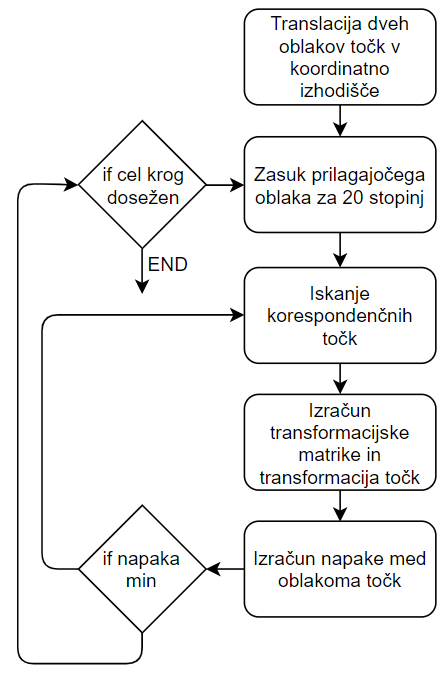
\includegraphics[width=4.5cm]{fig/alg_poravnava}}
	\caption{Potek algoritma poravnave.}
	\label{fig:alg_poravnava}
\end{figure}

\section{Zajem slik}
Sistem s katerim smo izvajali rekonstrukcijo je blokovno prikazan na sliki ~\ref{fig:blokovna}. Objekt, ki ga želimo skonstruirati postavimo na vrtljivo pozicionirno mizo. Iz zgornje strani navzdol svetimo s homogeno, difuzno osvetlitvijo. Objekta direktno ne osvetljujemo, saj je namen osvetlitve predvsem osvetlitev ozadja z enakomerno intenziteto. Cilj je doseči čimvečjo razliko v intenziteti med opazovanim objektom in zaslonom. Za ta namen je med objekt in svetilko postavljena svetlobna ovira. Slike smo zajemali z Raspberry Pi kamero v osi na objekt in na osvetljeno ozadje. Pred kamero je dodan filter za namen filtriranja okoliške svetlobe.

\begin{figure}[H]
	\centerline{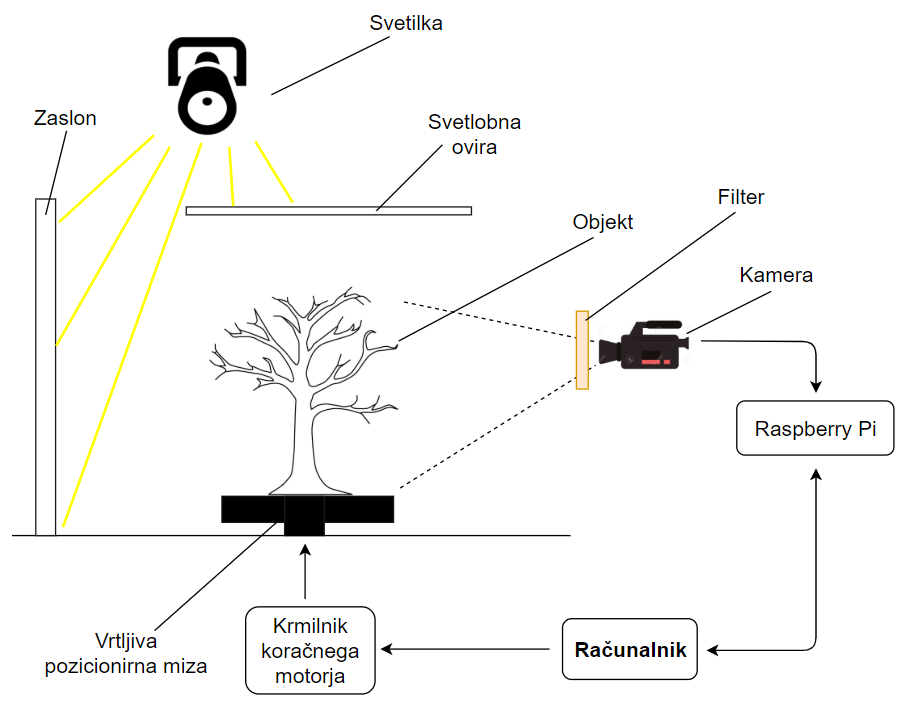
\includegraphics[width=8.2cm]{fig/blokovna_sistem}}
	\caption{Semioperacijska shema sistema.}
	\label{fig:blokovna}
\end{figure}
%
 Celoten proces zajemanja krmilnimo z računalnikom. Ta je žično povezan na krmilnik s katerim upravljamo rotirajočo pozicionirno mizo. Prav tako je računalnik brezžično povezan na Raspberry Pi. Ta zajete slike pošilja na računalnik. Objekt rekonstruiramo tako, da ga postavimo na predvideno mesto. Nato lahko pričnemo z zajemom slik. Najprej inicializiramo kamero na začetne vrednosti. Nastavimo ISO na 200, svetlost na 45 in resolucijo na 900x1000.  Objekt obračamo po začrtanih zasukih. Po vsakem izvedenem zasuku posnamemo eno sliko, ki se nato brezžično prenese iz Raspberry Pi-ja na računalnik. Postopek ponavljamo dokler objekta ne poslikamo v rangu celotnega kroga. Zajete slike ob znanih kotih zasuka se kasneje uporabijo za 3d rekonstrukcijo. V tabeli ~\ref{tab:komponente} so zapisane vse glavne komponente, ki so zajete v postavljenem sistemu. Manjše komponente kot so vijaki in nosilci v tabeli niso zajeti.

\begin{center}
	\centering
	\captionsetup{singlelinecheck = false, justification=justified}
	\captionof{table}{Komponente sistema.} 
	\label{tab:komponente} 
\begin{tabular}{|c|c|}
	\hline
	\textbf{Komponenta} & \textbf{Podrobnosti}                            \\ \hline
	Raspberry Pi        & Raspberry Pi 3 Model B                          \\ \hline
	Svetilka            & Halogenska svetilka (12V)            \\ \hline
	Zaslon              & Bela ravna plošča                               \\ \hline
	Krmilnik            & Fischertechnik stage control                \\ \hline
	Kamera              & RP Cam V2-8 MP,1080p \\ \hline
	Svetlobni filter    & Ozkopasovni filter         \\ \hline
	Svetlobna ovira     & Kartonasta zavesa                \\ \hline
		Pozicionirna miza   & Fischertechnik rotary stage                     \\ \hline
\end{tabular}
\end{center}
Primer zajete slike obravnavanega objekta z opisanim sistemom je prikazan na sliki ~\ref{fig:zajeta_slika}. S slike lahko vidimo dober kontrast objekta in precejšnjo razliko v barvi in svetlosti objekta proti ozadju. 

\begin{figure}[H]
	\centerline{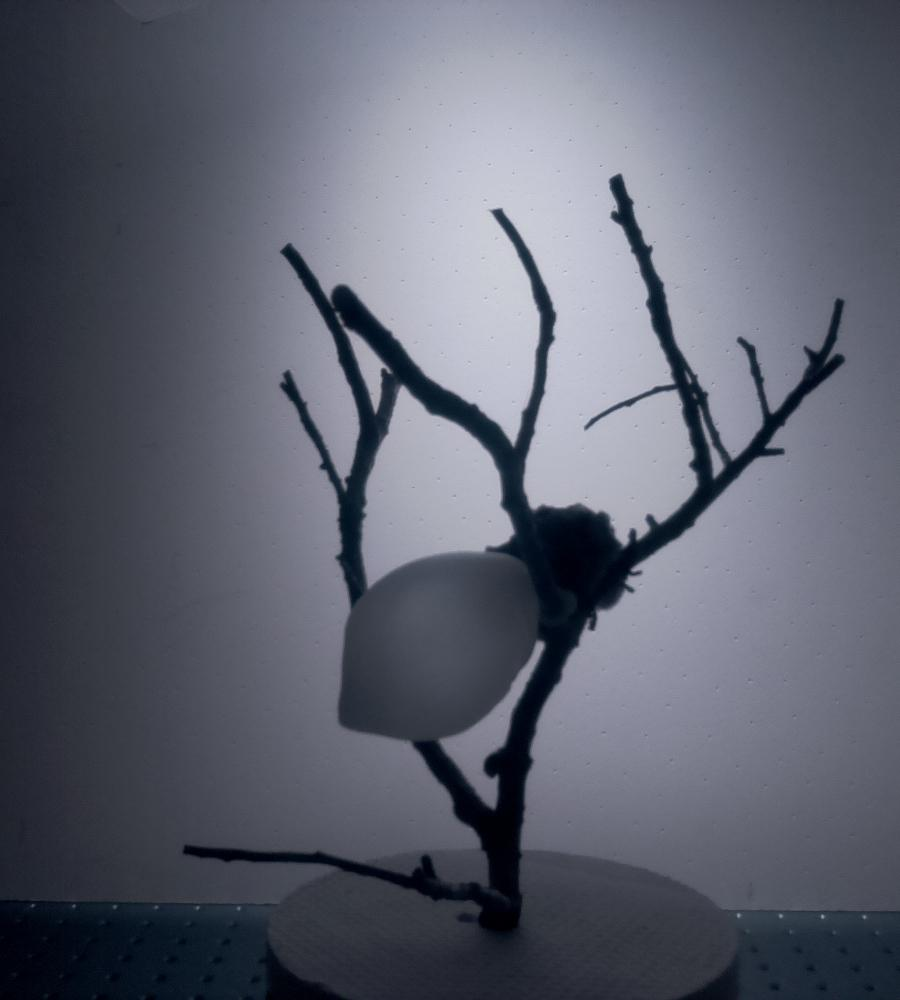
\includegraphics[width=4.2cm]{fig/zajeta_slika}}
	\caption{Zajeta slika.}
	\label{fig:zajeta_slika}
\end{figure}

\section{Rezultati}



\subsection{Vpliv kontrasta}
-  primerjava kompleksnosti modela
-  Primerjaj slab in dober kontrast slike (primer slusalk na 30 slikah)


\subsection{Število zajetih slik}
Dvakrat smo rekonstruirali isti predmet. Enkrat na podlagi 30 slik in drugič na podlagi 90 slik. Opazovali smo kako število zajetih slik vpliva na rekontrukcijo. Na sliki ~\ref{fig:slika_90_30} je čisto na levi strani prikazan skeniran objekt, na sredini objekt rekonstruiran na podlagi 90 slik in na desni objekt rekonstruiran na podlagi 30 slik. Vidimo, da je dobimo boljšo obliko na podlagi večih slik. Za prikaz celotnega objekta v obeh primerih bi bilo potrebno prilagoditi meje upragovanja. 
%
\begin{figure}[H]
	\centerline{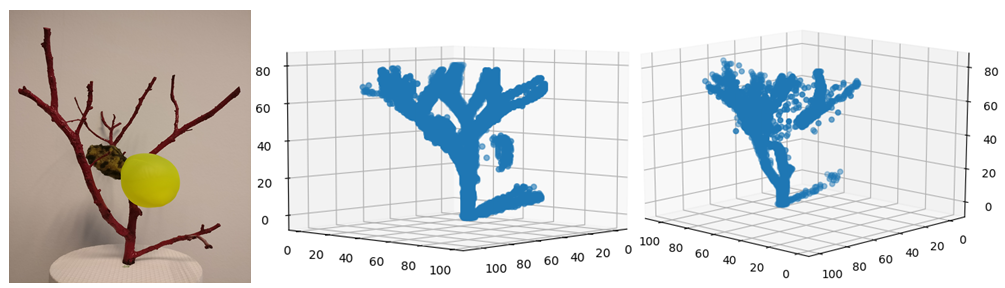
\includegraphics[width=8cm]{fig/slika_90_30}}
	\caption{a) objekt, b) skan - 90 slik, c) skan - 30 slik.}
	\label{fig:slika_90_30}
\end{figure}
%
%
\subsection{Poravnava oblakov točk}
Za dodaten eksperiment smo izvedli medsebojno poravnavo oblakov točk. Referenčni oblak točk smo zajeli z 90 slikami in si zapolnili referenčno lego objekta na pozicionirni mizi. Nato smo izvedli še šest zajemov po 30 slik. Ob vsakem zajemu smo skeniran objekt zasukali za predpisan kot glede na referenčno lego okoli vertikalne osi. Tako smo zajeli oblake točk zasukane za 45, 90, 135, 18, 225 in 315 stopinj. Na sliki ~\ref{fig:poravnava} sta zaradi preglednosti prikazana le referenčni oblak in oblak zasukan za 90 stopinj. Na levi strani sta oblaka prikazana pred poravnavo in na desni po poravnavi. 

\begin{figure}[H]
	\centerline{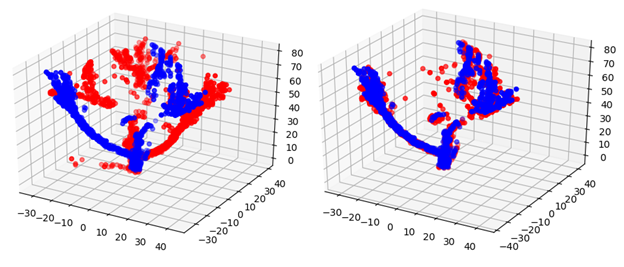
\includegraphics[width=8cm]{fig/poravnava}}
	\caption{a) neporavnana, b) poravnana.}
	\label{fig:poravnava}
\end{figure}
%
Za vse, pod različnimi koti zajete oblake točk, smo izvedli poravnavo. Nato smo iz pridobljene transformacijske matrike izluščili rotacijo okoli vertikalne osi. Ker smo poznali kote zasuka objekta glede na referenčno lego, smo jih primerjali s temi pridobljenimi iz transformacijske matrike. Na sliki ~\ref{fig:poravnava_graf} so z rdečo barvo prikazani ročno določeni zasuki, z modro pa zasuki pridobljeni iz transformacijske matrike.

\begin{figure}[H]
	\centerline{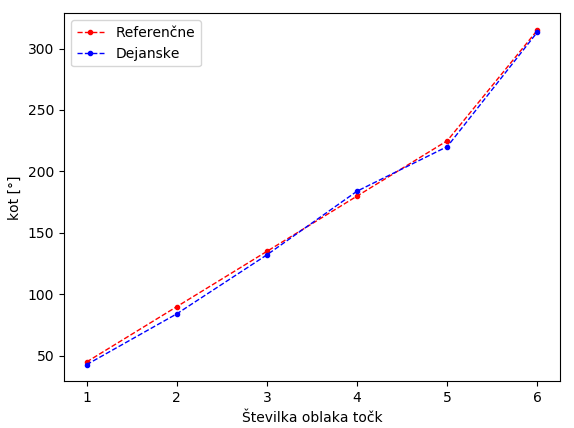
\includegraphics[width=8cm]{fig/graf_poravnave}}
	\caption{Razlika med referenčnimi in dejanskimi koti.}
	\label{fig:poravnava_graf}
\end{figure}

\subsection{Vzvratno inženirstvo}
-  mesh v blenderju in 3d print (reverse engineering)






\section{Zaključek}



\begin{thebibliography}{10}
\bibitem{kaeslin} H.~Kaeslin, {\em Digital integrated circuit design: from VLSI architectures to CMOS fabrication}, \hskip 1em plus 0.5em minus 0.4em \relax Cambridge University Press, 2008.

\bibitem{hspice} {\em HSPICE\textsuperscript{\textregistered} simulation and analysis user guide}, \hskip 1em plus 0.5em minus 0.4em \relax Synopsys\textsuperscript{\textregistered}, 2005.

\bibitem{kunderth} K.S.~Kunderth, {\em The designer's guide to SPICE and Spectre}, \hskip 1em plus 0.5em minus 0.4em \relax Kluwer Academic Publishers, 1995.

\bibitem{virtuoso} {\em Virtuoso\textsuperscript{\textregistered} Spectre\textsuperscript{\textregistered} circuit simulator user guide}, \hskip 1em plus 0.5em minus 0.4em \relax Cadence Design Systems, Inc., 2008.

\bibitem{tuma} T.~Tuma, \'{A}.~B\H{u}rmen, {\em Circuit simulation with SPICE Opus, theory and practice}, \hskip 1em plus 0.5em minus 0.4em \relax Birkh\"{a}user, 2009.

\bibitem{thomas} D.E.~Thomas, P.R.~Moorby, {\em The Verilog hardware description language}, 5\textsuperscript{th}~ed. \hskip 1em plus 0.5em minus 0.4em \relax Kluwer Academic Publishers, 2003.

\bibitem{pedroni} V.A.~Pedroni, {\em Circuit design with VHDL}, \hskip 1em plus 0.5em minus 0.4em \relax Massachusetts Institute of Technology, 2004.

\bibitem{kurup} P.~Kurup, T.~Abbasi, {\em Logic synthesis using Synopsys\textsuperscript{\textregistered}}, 2\textsuperscript{nd}~ed. \hskip 1em plus 0.5em minus 0.4em \relax Kluwer Academic Publishers, 1997.

\bibitem{bhatnagar} H.~Bhatnagar, {\em Advanced ASIC chip synthesis using Synopsys\textsuperscript{\textregistered} Design Compiler\texttrademark Physical Compiler\texttrademark and PrimeTime\textsuperscript{\textregistered}}, 2\textsuperscript{nd}~ed. \hskip 1em plus 0.5em minus 0.4em \relax Kluwer Academic Publishers, 2002.

\bibitem{burmen1} \'{A}.~B\H{u}rmen et al., ``Automated robust design and optimization of integrated circuits by means of penalty functions,'' \hskip 1em plus 0.5em minus 0.4em \relax {\em AE\"{U}, International Journal of Electronics and Communications}, vol. 57, no. 1, pp. 47--56, 2003.

\bibitem{olensek} J.~Olen\v{s}ek, \'{A}.~B\H{u}rmen, J.~Puhan, T.~Tuma, ``DESA: a new hybrid global optimization method and its application to analog integrated circuit sizing,'' \hskip 1em plus 0.5em minus 0.4em \relax {\em Journal of Global Optimization}, vol. 44, no. 1, pp. 1--25, 2008.

\bibitem{hooke} R.~Hooke, T.~Jeeves, ``Direct search solutions of numerical and statistical problems,'' \hskip 1em plus 0.5em minus 0.4em \relax {\em Journal of the Association for Computing Machinery}, vol. 8, no. 2, pp. 212--229, 1961.

\bibitem{burmen2} \'{A}.~B\H{u}rmen, I.~Fajfar, T.~Tuma, ``Combined Simplex-Trust-Region optimization algorithm for automated IC design,'' \hskip 1em plus 0.5em minus 0.4em \relax {\em Proceedings of ECCTD07 European Conference on Circuit Theory and Design}, pp. 543--546, 2007.
\end{thebibliography}



\vfill

\label{finish}

% that's all folks
\end{document}


